\documentclass[11pt]{article}
\usepackage[T1]{fontenc}
\usepackage{lmodern}
\input{glyphtounicode}
\input{glyphtounicode-cmex}
\pdfgentounicode=1
\pdfglyphtounicode{negationslash}{0338}
\usepackage[margin=1.08in]{geometry}
\usepackage{amsmath,amssymb,amsthm,mathtools}
\usepackage{microtype}
\usepackage{enumitem}
\usepackage{needspace}
\usepackage{xcolor}
\usepackage{tikz}
\usetikzlibrary{arrows.meta}
\usepackage[colorlinks=true,linkcolor=blue!45!black,citecolor=blue!45!black,urlcolor=blue!45!black]{hyperref}
\usepackage[nameinlink,capitalise,noabbrev]{cleveref}
\numberwithin{equation}{section}
\newtheorem{theorem}{Theorem}[section]
\newtheorem{lemma}[theorem]{Lemma}
\newtheorem{proposition}[theorem]{Proposition}
\newtheorem{corollary}[theorem]{Corollary}
\theoremstyle{remark}
\newtheorem{remark}[theorem]{Remark}
\AddToHook{env/theorem/before}{\Needspace{5\baselineskip}}
\AddToHook{env/lemma/before}{\Needspace{5\baselineskip}}
\AddToHook{env/proposition/before}{\Needspace{5\baselineskip}}
\AddToHook{env/corollary/before}{\Needspace{5\baselineskip}}
\AddToHook{env/remark/before}{\Needspace{5\baselineskip}}
\newcommand{\R}{\mathbb R}
\newcommand{\C}{\mathbb C}
\newcommand{\D}{\mathbb D}
\newcommand{\Sone}{\mathbb S^1}
\newcommand{\V}{\mathcal V}
\newcommand{\HH}{\mathcal H}
\newcommand{\Q}{\mathcal Q}
\newcommand{\dd}{\,\mathrm d}
\newcommand{\grad}{\nabla}
\newcommand{\curl}{\operatorname{curl}}
\newcommand{\diver}{\operatorname{div}}
\newcommand{\tr}{\operatorname{tr}}
\newcommand{\ip}[2]{\langle #1,#2\rangle}
\newcommand{\norm}[1]{\lVert #1\rVert}
\newcommand{\one}{\mathbf 1}
\newcommand{\supp}{\operatorname{supp}}
\newcommand{\PSD}{\succeq0}
\DeclareMathOperator{\spanop}{span}
\setlist{topsep=5pt,itemsep=3pt}
\setlength{\emergencystretch}{2em}
\title{Strict hot spots and absence of interior critical points on smooth simply connected planar domains}
\author{OpenAI}
\date{September 24, 2026}
\hypersetup{
  pdftitle={Strict hot spots and absence of interior critical points on smooth simply connected planar domains},
  pdfauthor={OpenAI}
}
\begin{document}
\maketitle
\begin{abstract}
We prove the strict hot spots conjecture for smooth bounded simply connected planar domains. More precisely, every nonzero eigenfunction for the first positive Neumann eigenvalue has nonvanishing gradient in the interior, so all its global maxima and minima lie on the boundary. This holds even when the eigenvalue is multiple.
\end{abstract}
\section{Introduction}

The hot-spots problem arose from Rauch's discussion of the long-time behavior of heat flow with insulating boundary conditions \cite{Rauch1975}. Its spectral formulation asks whether the extrema of a first-positive Neumann eigenfunction occur on the boundary. Bañuelos and Burdzy distinguished strict and nonstrict formulations, and assertions about every eigenfunction from the existence of one favorable eigenfunction \cite{BanuelosBurdzy1999}. These distinctions matter when the eigenvalue is multiple.

Let $\Omega\subset\R^2$ be a nonempty bounded simply connected open set with $C^\infty$ boundary. In particular, $\Omega$ is connected. Set
\begin{equation}\label{eq:mu}
\mu=\mu_1(\Omega)
=\inf_{\substack{0\ne v\in H^1(\Omega)\\ \int_\Omega v=0}}
\frac{\int_\Omega|\grad v|^2}{\int_\Omega|v|^2},
\end{equation}
and let $\V$ be the real Neumann eigenspace for $\mu$. We count only positive eigenvalues in this notation; sources that count the constant eigenfunction first write $\mu_2$ for this same eigenvalue.

\begin{theorem}\label{thm:main}
For every $0\ne u\in\V$,
\[
\grad u(x)\ne0\qquad(x\in\Omega).
\]
In particular,
\begin{equation}\label{eq:hotspots}
\min_{y\in\partial\Omega}u(y)<u(x)<\max_{y\in\partial\Omega}u(y)
\qquad(x\in\Omega).
\end{equation}
\end{theorem}

The theorem imposes no convexity or symmetry condition. It applies to every member of the first positive eigenspace, including when the eigenvalue is multiple. The nonvanishing-gradient conclusion is stronger than \eqref{eq:hotspots}, since it also rules out interior saddle points.

\paragraph{Background and methods.}
Topology matters in the hot-spots problem. Burdzy and Werner constructed a planar counterexample with two holes and a simple first-positive eigenvalue \cite{BurdzyWerner1999}. Bass and Burdzy obtained examples with both extrema strictly in the interior \cite{BassBurdzy2000}, and Burdzy subsequently obtained this behavior with just one hole \cite{Burdzy2005}. The simply connected planar conjecture is stated explicitly in \cite[Conjecture~1.2(ii)]{Burdzy2005}.

Important geometric special cases already establish strong gradient conclusions. Jerison and Nadirashvili proved a positive directional derivative for every first-positive eigenfunction on convex planar domains with two orthogonal reflection symmetries, allowing multiple eigenvalues \cite[Theorem~1.4]{JerisonNadirashvili2000}. Probabilistic coupling methods developed by Bañuelos and Burdzy \cite{BanuelosBurdzy1999} led to further results. Pascu proved boundary-only extrema for antisymmetric eigenfunctions on $C^{1,\alpha}$ convex planar domains with one reflection symmetry, where $0<\alpha<1$ \cite{Pascu2002}. Atar and Burdzy treated every first-positive eigenfunction on lip domains, a class of Lipschitz domains bounded between graphs of functions with Lipschitz constants at most one \cite{AtarBurdzy2004}. Miyamoto obtained interior critical-point exclusion under a spectral-diameter condition, giving nonsymmetric nearly circular convex examples \cite[Lemma~1.2 and Theorem~A]{Miyamoto2007}.

The polygonal problem has a complementary development. Siudeja proved hot-spots results for a class of acute triangles \cite{Siudeja2015}. Judge and Mondal, with their subsequent erratum, excluded interior critical points for every first-positive Neumann eigenfunction on every Euclidean triangle \cite{JudgeMondal2020,JudgeMondal2022}. Chen, Gui and Yao established the finer classification of nonvertex critical points \cite{ChenGuiYao2026}. These results concern domains with corners; \Cref{thm:main} concerns the full smooth simply connected planar class.

Recent quantitative work measures how far the hot-spots conclusion can fail. For general bounded connected Lipschitz domains, de Dios Pont, Hsu and Taylor determined the sharp dimension-dependent upper bound for the ratio of a first-positive Neumann eigenfunction's supremum over the domain to its maximum on the boundary \cite[Definition~1 and Theorem~4]{deDiosPontHsuTaylor2025}. Deng, Jiang and Yang obtained quantitative bounds for convex domains in two-dimensional space forms \cite{DengJiangYang2026}. Such ratios concern extrema; excluding every interior critical point also requires excluding saddle points.

Our starting point is Rohleder's variational principle for tangent vector fields \cite{Rohleder2021,Rohleder2024}. In its lip-domain application, taking componentwise absolute values after a suitable rotation preserves the required tangent boundary condition and yields directional monotonicity. We use scalar boundary multipliers to keep tangency on an arbitrary smooth boundary, and construct those multipliers through a reciprocal Green-kernel theorem.

The difficulty is to control the gradient without a preferred direction in the domain. Each Cartesian derivative of an eigenfunction solves the same Helmholtz equation, but its boundary values need not have a fixed sign. The Neumann condition instead constrains the two derivatives together: their vector is tangent to the boundary. We use that constraint through a nonnegative quadratic form whose nullspace consists exactly of first-positive eigenfunction gradients. The remaining task is to construct enough scalar boundary multipliers that preserve this nullspace if an interior critical point exists.

\paragraph{The mechanism.}
Write $\D=\{z\in\C:|z|<1\}$ and $\Sone=\partial\D$, and let $\Phi:\D\to\Omega$ be a smooth conformal parametrization. The proof begins with the variational principle for tangent vector fields associated with Neumann gradients. For a tangent vector field $X$, its divergence--curl energy is at least $\mu\norm{X}_2^2$, with equality exactly for gradients of functions in $\V$. After this conformal change of variables, solving the scalar Helmholtz equation in each Cartesian component gives a nonnegative quadratic form $E$ on boundary vector data. If $g$ is the boundary gradient of an eigenfunction, then $E(g)=0$, and a scalar multiplier $b$ satisfies
\[
E(bg)=\frac12\iint_{\Sone\times\Sone}
N(s,t)(b(s)-b(t))^2g(s)\cdot g(t)\dd s\dd t.
\]
Here $N$ is a positive boundary kernel, and the corresponding interior evaluation kernel is denoted by $K$.

The sign of $g(s)\cdot g(t)$ prevents a direct positivity argument in this identity. The main kernel result supplies a family of multipliers whose squared differences remove the factor $N$. For every interior point $p$,
\[
D_p(s,t)=\frac{K(p,s)K(p,t)}{N(s,t)}\quad(s\ne t),
\qquad D_p(s,s)=0,
\]
is conditionally negative semidefinite. It is therefore the squared distance of an injective Lipschitz map from the circle to a real Hilbert space. Applying the preceding energy identity to its coordinates gives
\[
\sum_j E(b_jg)=\frac12|\grad u(\Phi(p))|^2.
\]
A critical point would thus produce too many eigenfunction gradients, contradicting the planar multiplicity bound or boundary uniqueness.

The construction of $D_p$ is the central analytic step. We first regularize the disk Green function so that the entrywise reciprocal of every finite kernel matrix has at most one positive eigenvalue. This property survives successive rank-one updates along columns of the current kernel matrix, which sum the Green resolvent over a finite set of integration nodes. Positive quadrature and monotone limits then pass from those matrices to the singular Green kernel and finally to its boundary kernels. Taking the boundary limit before removing a compact-support cutoff avoids treating a Poisson kernel as an $L^2$ function when it need not be one.

The kernel theorem, \Cref{thm:negative-kernel}, holds for every bounded nonnegative disk potential satisfying the subcritical Dirichlet inequality \eqref{eq:subcritical}, independently of the conformal origin of that potential. The reciprocal-matrix condition comes from the McCullough--Quiggin characterization of complete Nevanlinna--Pick kernels \cite{McCullough1992,McCullough1994,Quiggin1993,Quiggin1994}; see also \cite[Corollary~1.12]{AglerMcCarthy2000}. Schoenberg's squared-distance correspondence supplies the Hilbert-space realization \cite{Schoenberg1938}. The analytic work here concerns the singular Green kernel, its positive-potential resolvent, and its boundary limit; the resulting theorem can be used independently of the eigenfunction argument.

\paragraph{Organization and background.}
\Cref{sec:preliminaries} proves the spectral gap, the smooth conformal reduction, and the multiplicity bound. \Cref{sec:vector} proves the vector variational principle. \Cref{sec:boundary} constructs the boundary kernels and derives the multiplier identity. \Cref{sec:reciprocal} proves their conditional negativity, and \Cref{sec:conclusion} completes the argument.
We use standard Sobolev compactness, Poincar\'e and trace inequalities on smooth bounded domains, Poisson solvability and elliptic boundary regularity, the maximum and boundary point principles, elementary complex analysis, and planar separation. All specialized ingredients used in the proof are established below. The smooth-boundary regularity input is \cite[Chapter~III, Theorems~6.1, 6.4 and~6.5]{Showalter1994}: $L^2$ Poisson data give $H^2$ solutions under homogeneous Dirichlet or Neumann conditions, and higher regularity follows with smoother data. Subtracting a smooth extension handles the inhomogeneous Dirichlet data used below. Bootstrap and Sobolev embedding make weak Neumann eigenfunctions smooth up to the boundary. Interior solutions of $(\Delta+\mu)v=0$ are analytic; alternatively, $e^{\sqrt\mu t}v(x)$ is harmonic in one additional variable.

\section{Spectral and planar preliminaries}\label{sec:preliminaries}

Write $\lambda_D$ for the first Dirichlet eigenvalue of $\Omega$. Both $\mu$ and $\lambda_D$ are positive by the respective Poincar\'e inequalities. Their Rayleigh infima are attained by compactness, and the eigenspaces are finite-dimensional.

The strict separation below is the first-mode case of the Friedlander--Filonov comparison \cite{Friedlander1991,Filonov2005}. We give the plane-wave argument of Filonov in the form needed here, including the strictness that identifies the equality space of the later vector variational principle.

\begin{lemma}\label{lem:gap}
One has $\mu<\lambda_D$.
\end{lemma}
\begin{proof}
Choose a nonzero nonnegative Dirichlet minimizer $\phi$, using absolute values in the Rayleigh quotient. Then $\int_\Omega\phi>0$. Work temporarily over $\C$. For $k\in\R^2$ with $|k|^2=\lambda_D$, put
\[
e_k(x)=e^{ik\cdot x},\qquad
w_k=e_k-\frac{\int_\Omega e_k}{\int_\Omega\phi}\phi.
\]
Each $w_k$ has mean zero. The form $\int(|\grad v|^2-\lambda_D|v|^2)$ vanishes on $e_k$ and $\phi$; its cross term vanishes because $-\Delta e_k=\lambda_De_k$ and $\phi$ has zero trace. Thus every nonzero $w_k$ has Rayleigh quotient $\lambda_D$, proving $\mu\le\lambda_D$.

If equality held, each such $w_k$ would be a Neumann eigenfunction by variational equality. The Euler equation first holds against mean-zero tests and then against all tests, since $w_k$ has mean zero. But distinct plane waves are linearly independent: restrict any finite family to a line segment in an interior ball whose direction gives distinct frequencies. Subtracting multiples of one fixed function leaves their span infinite-dimensional. This contradicts finite eigenspace dimension. The real Neumann inequality and its equality case apply in the complexified space by separating real and imaginary parts.
\end{proof}

We also include the smooth conformal parametrization used throughout the proof; see \cite{Pommerenke1992} for the classical boundary-regularity theory of conformal maps.

\begin{lemma}\label{lem:conformal}
There is a conformal bijection $\Phi:\D\to\Omega$ extending to a smooth diffeomorphism of closures, with $\Phi'\ne0$ on $\overline\D$.
\end{lemma}
\begin{proof}
Identify the plane with $\C$ and fix $a\in\Omega$. Let $l$ solve the harmonic Dirichlet problem with boundary values $\log|z-a|$. It is smooth up to the boundary. Simple connectivity gives a harmonic conjugate $\widetilde l$; its gradient extends smoothly, so the conjugate also extends smoothly in boundary charts. The holomorphic function
\[
m(z)=(z-a)\exp(-l(z)-i\widetilde l(z))
\]
has modulus one on the boundary, modulus less than one inside, and precisely one zero, of order one. Near the boundary, $\log|m|$ is harmonic, negative inside, and zero on the boundary. The boundary point lemma gives a nonzero normal derivative, so $m'$ does not vanish there.

For any $w\in\D$, take a smooth inner approximation of $\Omega$ so close to its boundary that $|m|>|w|$ throughout the omitted collar. Rouch\'e's theorem gives exactly one zero of $m-w$ in that approximation, counting multiplicity, because $m$ has exactly one. There are none in the collar. Thus $m$ is a biholomorphism in the interior. It maps the boundary onto the circle by compactness. Its local boundary inverses imply injectivity there: two boundary preimages would give two nearby interior preimages. The inverse map is the required $\Phi$.
\end{proof}

Throughout, $\Sone=\partial\D$ carries arclength $\dd s$, of total mass $2\pi$.

To bound the dimension of $\V$, we transfer its mean-zero condition to the boundary and use connectedness of the positive and negative sets to control boundary signs.

\begin{lemma}\label{lem:boundary-weight}
There is a fixed smooth positive function $\beta$ on $\Sone$ such that every $v\in\V$ has boundary trace $h_v=v\circ\Phi$ satisfying
\[
\int_{\Sone}\beta h_v\dd s=0.
\]
If $v\ne0$, its boundary trace is nonzero and takes both signs.
\end{lemma}
\begin{proof}
By \Cref{lem:gap}, the Dirichlet problem
\[
(-\Delta-\mu)L=1,\qquad L|_{\partial\Omega}=0
\]
is coercive and has a smooth solution. Testing by its negative part gives $L\ge0$. Hence $-\Delta L=1+\mu L>0$, and the boundary point lemma gives $-\partial_\nu L>0$. Green's identity and the Neumann equation yield
\[
0=\int_\Omega v=-\int_{\partial\Omega}v\,\partial_\nu L
=\int_{\Sone}\beta(s)h_v(s)\dd s,
\quad
\beta=|\Phi'|\,(-\partial_\nu L)\circ\Phi.
\]
If $h_v=0$, then $v\in H^1_0(\Omega)$, and the Dirichlet inequality and $\mu<\lambda_D$ force $v=0$. Positivity of $\beta$ gives the last assertion.
\end{proof}

\begin{lemma}\label{lem:nodal}
For $0\ne v\in\V$, the sets $\{v>0\}$ and $\{v<0\}$ are connected. Its boundary trace cannot have four cyclically ordered points with strictly alternating signs.
\end{lemma}
\begin{proof}
For each component $U$ of a sign set, the function $v_U=v\one_U$ belongs to $H^1(\Omega)$ and has weak gradient $\one_U\grad v$. Indeed it is locally Lipschitz in interior balls: any transition between $U$ and its complement crosses a zero of $v$, so the local Lipschitz bound for $v$ also bounds the zeroed function. This gives the local weak-gradient identity, and the global $L^2$ bounds give global $H^1$ membership. Testing the eigenfunction equation by $v_U$ shows
\[
\int_\Omega|\grad v_U|^2=\mu\int_\Omega|v_U|^2.
\]
If at least three sign components existed, a nonzero linear combination of two restrictions could be chosen mean zero. Disjoint supports show that it attains the quotient $\mu$. It is therefore an eigenfunction, but vanishes on the omitted open component, contradicting interior analyticity. Both sign sets are nonempty, so each is connected.

Four alternating strict signs on the boundary would give a simple arc joining the two positive points, otherwise in the positive interior set, and another joining the negative points in the negative interior set. Such arcs exist by connectedness of open planar sign sets, using short interior end segments and then polygonal paths with loops removed. After applying $\Phi^{-1}$, their endpoints alternate on a circle. Planar separation forces the two arcs to intersect, contrary to their signs; see \Cref{fig:boundary-signs}.
\end{proof}

\begin{figure}[htbp]
  \centering
  \begin{minipage}{.84\textwidth}
  \centering\small
  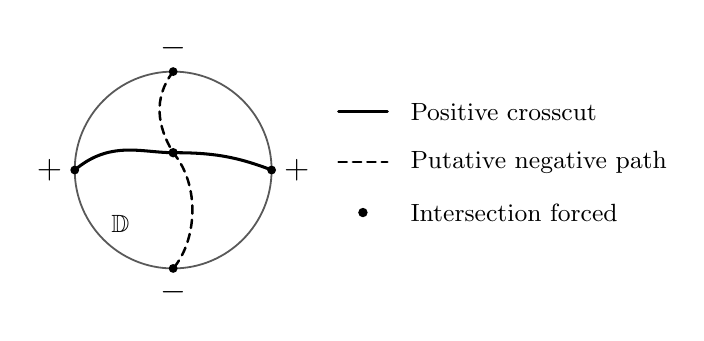
\begin{tikzpicture}[x=1cm,y=1cm,font=\small,
      line cap=round,line join=round]
    \draw[black!65,line width=.65pt] (0,0) circle[radius=1.25];
    \node at (-.67,-.69) {$\D$};

    \draw[line width=1.1pt]
      (-1.25,0) .. controls (-.8,.38) and (-.4,.22) .. (0,.22)
      .. controls (.48,.22) and (.78,.18) .. (1.25,0);

    \draw[line width=.9pt,dash pattern=on 3pt off 2.2pt]
      (0,1.25) .. controls (-.26,.91) and (-.20,.55) .. (0,.22)
      .. controls (.35,-.20) and (.30,-.90) .. (0,-1.25);
    \fill (0,.22) circle[radius=1.7pt];

    \foreach \x/\y in {-1.25/0,1.25/0,0/1.25,0/-1.25}
      \fill (\x,\y) circle[radius=1.6pt];
    \node[font=\large] at (-1.57,0) {$+$};
    \node[font=\large] at (1.57,0) {$+$};
    \node[font=\large] at (0,1.55) {$-$};
    \node[font=\large] at (0,-1.55) {$-$};

    \draw[line width=1.1pt] (2.10,.74) -- (2.72,.74);
    \node[anchor=west] at (2.89,.74) {Positive crosscut};
    \draw[line width=.9pt,dash pattern=on 3pt off 2.2pt]
      (2.10,.10) -- (2.72,.10);
    \node[anchor=west] at (2.89,.10) {Putative negative path};
    \fill (2.41,-.54) circle[radius=1.7pt];
    \node[anchor=west] at (2.89,-.54) {Intersection forced};
  \end{tikzpicture}
  \caption{Connectedness of the positive set gives a crosscut joining the
  $+$ points. It separates the two $-$ points, forcing any negative connecting
  path to meet it. The dashed path illustrates this contradiction; all four
  boundary signs are strict.}
  \label{fig:boundary-signs}
  \end{minipage}
\end{figure}


\Needspace{7\baselineskip}
The following multiplicity bound is due to Nadirashvili \cite[Theorem~3, p.~227]{Nadirashvili1988}; see also \cite[Proposition~2.5]{BanuelosBurdzy1999}. The boundary-sign proof is included for completeness.

\begin{proposition}\label{prop:multiplicity}
The real eigenspace $\V$ has dimension at most two.
\end{proposition}
\begin{proof}
Suppose its dimension is at least three. Since the trace map is injective, choose $0\ne v\in\V$ whose trace $h=h_v$ satisfies
\[
\int_{\Sone}\beta h\cos\theta\dd s
=\int_{\Sone}\beta h\sin\theta\dd s=0,
\qquad s=e^{i\theta}.
\]
It is already orthogonal to $1$ by \Cref{lem:boundary-weight}. Cut the circle at a strictly negative point and write its angles as $(\theta_0,\theta_0+2\pi)$. If $a$ and $b$ are the infimum and supremum of the positive angles, then
\[
\theta_0<a<b<\theta_0+2\pi.
\]
There are no positive values outside $[a,b]$. Nor is there a negative value between $a$ and $b$: positive values on either side of it, together with the cut point, would violate \Cref{lem:nodal}. The function
\[
F(\theta)=\cos\!\left(\theta-\frac{a+b}{2}\right)
-\cos\!\left(\frac{b-a}{2}\right)
\]
is strictly positive on $(a,b)$ and negative outside $[a,b]$ in the cut interval. Consequently $Fh\ge0$ everywhere and $Fh>0$ on a nonempty open set. Thus $\int\beta Fh>0$, contradicting the three orthogonalities.
\end{proof}

\section{A variational principle for tangent vector fields}\label{sec:vector}

For a real vector field $X\in H^1(\Omega;\R^2)$ with tangent trace, meaning $\tr X\cdot\nu=0$, set
\[
\Q(X)=\int_\Omega\bigl(|\diver X|^2+|\curl X|^2\bigr),
\qquad \curl X=\partial_1X_2-\partial_2X_1.
\]
The following is Rohleder's vector variational principle \cite[Theorem~1.1]{Rohleder2021}; see also \cite{Rohleder2024}. We include its derivation, in particular its equality case. Our curvature convention below is the opposite of his, so the corresponding boundary term has the opposite sign.

\begin{proposition}\label{prop:vector}
For every such $X$,
\begin{equation}\label{eq:vector-inequality}
\Q(X)\ge\mu\int_\Omega|X|^2,
\end{equation}
with equality exactly when $X=\grad v$ for some $v\in\V$.
\end{proposition}
\begin{proof}
Solve
\[
\Delta v=\diver X,\quad \partial_\nu v=0,\quad\int_\Omega v=0,
\qquad
\Delta j=\curl X,\quad j|_{\partial\Omega}=0.
\]
The Neumann compatibility follows from the tangent trace. The solutions are in $H^2(\Omega)$ by smooth-boundary regularity \cite[Chapter~III, Theorems~6.1 and~6.4]{Showalter1994}. The rotated gradient $\grad^\perp j=(-\partial_2j,\partial_1j)$ is tangent. Thus
\[
Z=X-\grad v-\grad^\perp j
\]
is tangent, curl-free, and divergence-free. Its components are harmonic in the interior, so $Z$ is smooth there. Simple connectivity gives an interior potential $r$ with $Z=\grad r$.

Here $r\in H^1(\Omega)$, as can be seen without assuming its global integrability in advance. For $M>0$, its bounded truncation $r_M=\max(-M,\min(r,M))$ has local weak gradient of norm at most $|Z|$, hence belongs globally to $H^1(\Omega)$. Fix an interior ball $B$. Its averages $(r_M)_B$ are bounded by $\sup_B|r|$. The Poincar\'e inequality, with this fixed-ball average as anchor, gives
\[
\norm{r_M}_{L^2(\Omega)}
\le C\norm{\grad r_M}_{L^2(\Omega)}+C|(r_M)_B|
\le C\norm Z_2+C\sup_B|r|.
\]
Fatou gives $r\in L^2$, and its weak gradient is $Z$. Testing $\diver Z=0$ against $r$, with its zero normal trace, yields $\int|\grad r|^2=0$. Thus
\[
X=\grad v+\grad^\perp j.
\]
The summands are orthogonal in $L^2$, since the second is divergence-free and tangent. Moreover,
\[
\Q(X)=\norm{\Delta v}_2^2+\norm{\Delta j}_2^2.
\]
Integration by parts and the two Poincar\'e inequalities show
\[
\norm{\grad v}_2^2
\le\norm v_2\norm{\Delta v}_2
\le\mu^{-1/2}\norm{\grad v}_2\norm{\Delta v}_2,
\]
and likewise $\norm{\Delta j}_2^2\ge\lambda_D\norm{\grad j}_2^2$. Hence
\[
\Q(X)\ge\mu\norm{\grad v}_2^2+\lambda_D\norm{\grad j}_2^2
=\mu\norm X_2^2+(\lambda_D-\mu)\norm{\grad j}_2^2.
\]
By \Cref{lem:gap}, this proves \eqref{eq:vector-inequality}. Equality forces $j=0$ and equality in the Rayleigh inequality for $v$, so $v\in\V$. Conversely, gradients of functions in $\V$ give equality directly.
\end{proof}

For a differential-form interpretation of this divergence--curl energy, see \cite[Section~5.1]{FriesGoffengMiranda2026}. We will use the following boundary identity in the fixed Cartesian coordinates of the plane.

Let $\tau$ be the counterclockwise unit tangent to $\partial\Omega$, and put
\[
\kappa=\det(\tau,\partial_\tau\tau).
\]
Thus $\kappa$ is positive on a convex circle.

\begin{lemma}\label{lem:curvature}
For tangent $X\in H^1(\Omega;\R^2)$,
\begin{equation}\label{eq:curvature}
\Q(X)=\int_\Omega|\grad X|^2
+\int_{\partial\Omega}\kappa|X|^2.
\end{equation}
\end{lemma}
\begin{proof}
For smooth fields, the difference of the bulk integrands is $2\det\grad X$. Its integral is the boundary pairing
\[
\int_{\partial\Omega}
(X_1\partial_\tau X_2-X_2\partial_\tau X_1).
\]
This identity extends to $H^1$ fields by smooth approximation, since traces are in $H^{1/2}$ and their tangential derivatives are in $H^{-1/2}$. If the trace is $a\tau$, the pairing is $\int\kappa a^2$. This follows first for smooth $a$ and then by approximation in $H^{1/2}$. It gives \eqref{eq:curvature}.
\end{proof}

\section{Boundary kernels and the multiplier identity}\label{sec:boundary}

Our objective is a boundary formula for the nonnegative vector energy from \Cref{prop:vector}. We first construct scalar solution and interaction kernels for a general nonnegative subcritical potential on the disk. We then return to the conformal potential and derive the multiplier identity that will connect these kernels to an eigenfunction gradient.

\subsection{A subcritical disk potential}

The conformal map of \Cref{lem:conformal} defines a measure
\begin{equation}\label{eq:q}
\dd q(x)=\mu|\Phi'(x)|^2\dd x.
\end{equation}
It has a bounded positive density. A subscript $q$ on an inner product or norm denotes $L^2(q)$. Conformal invariance of the Dirichlet integral and the Dirichlet inequality on $\Omega$ give
\begin{equation}\label{eq:subcritical}
\norm\psi_{L^2(q)}^2\le d\int_\D|\grad\psi|^2,
\qquad \psi\in H^1_0(\D),\qquad d=\frac\mu{\lambda_D}<1.
\end{equation}
Until the vector-form application in \Cref{subsec:energy}, only boundedness and nonnegativity of the density and \eqref{eq:subcritical} are needed. In particular, the kernel constructions apply to any measure $q$ with those properties.
For such a general measure we fix a constant $0<d<1$ satisfying the same inequality; the zero measure also admits this choice.

The Dirichlet Green function and Poisson kernel of the disk are
\begin{align}
G(x,y)&=\frac1{2\pi}\log\left|\frac{1-x\overline y}{x-y}\right|
=\frac1{4\pi}\log\left(1+\frac{(1-|x|^2)(1-|y|^2)}{|x-y|^2}\right),\label{eq:green}\\
P_s(x)&=\frac{1-|x|^2}{2\pi|s-x|^2},\qquad s\in\Sone.\label{eq:poisson}
\end{align}
The Green function is positive and is assigned value $+\infty$ on the diagonal. Its logarithmic pole, harmonic correction, and zero boundary data give the Green identity. Also $\int_{\Sone}P_s(x)\dd s=1$.

\begin{lemma}\label{lem:green-operator}
The operator
\[
Tf(x)=\int_\D G(x,y)f(y)\dd q(y)
\]
is a bounded self-adjoint operator on $L^2(q)$ with $\norm T\le d<1$. The same statement holds with $q$ replaced by any measure $0\le\rho\le q$.
\end{lemma}
\begin{proof}
Write $\dd q=a\dd x$, with $a$ bounded. For $f\in L^2(q)$, the source $af$ lies in $L^2(\dd x)$, since $\int|af|^2\le\norm a_\infty\int|f|^2\dd q$. Its Dirichlet solution $\psi=Tf$ satisfies
\[
\int_\D|\grad\psi|^2=\ip{\psi}{f}_q.
\]
Combining this with \eqref{eq:subcritical} gives
\[
\norm\psi_q^2\le d\norm\psi_q\norm f_q,
\]
hence the norm bound. Symmetry follows from the Green kernel, or by testing the two Poisson equations against each other. The Green formula can first be proved for smooth compactly supported sources and then passed to $L^2(\dd x)$ by approximation; $G(x,\cdot)\in L^2(\dd x)$ gives pointwise evaluation. These sections vary continuously in $L^2$ on compact interior sets, so this is the continuous interior representative. For $\rho\le q$, its density remains bounded and its weighted Dirichlet inequality follows from \eqref{eq:subcritical}, proving the same result.
\end{proof}

For Lipschitz scalar or vector boundary data $h$, let
\[
Ah(x)=\int_{\Sone}P_s(x)h(s)\dd s.
\]
This harmonic extension belongs to $H^1(\D)$. The unique weak solution with trace $h$ of
\[
-\Delta W_h\dd x=W_h\dd q
\]
is
\begin{equation}\label{eq:extension}
W_h=Ah+T(I-T)^{-1}Ah.
\end{equation}
Indeed the correction has zero trace and solves the required Poisson equation. Uniqueness follows from \eqref{eq:subcritical}. The construction is componentwise for vectors.

\subsection{Positive kernels and their estimates}

For $p\in\D$ and distinct $s,t\in\Sone$, define
\begin{align}
K(p,s)&=P_s(p)+\sum_{n\ge1}(T^nP_s)(p),\label{eq:K}\\
R(s,t)&=\sum_{n\ge0}\int_\D P_s\,T^nP_t\dd q,\label{eq:R}\\
N(s,t)&=N_0(s,t)+R(s,t),\qquad N_0(s,t)=\frac1{\pi|s-t|^2}.\label{eq:N}
\end{align}
Powers applied to $P_s$ mean iterated nonnegative kernel integrals, not an a priori application of an $L^2$ operator to $P_s$.

\begin{lemma}\label{lem:kernel-estimates}
The kernels above are finite at the stated points. For fixed $p$, $K(p,\cdot)$ is positive and bounded. The kernel $R$ is symmetric, nonnegative, and integrable on $\Sone\times\Sone$, with
\begin{equation}\label{eq:R-integral}
\iint R(s,t)\dd s\dd t\le\frac{q(\D)}{1-d}.
\end{equation}
For Lipschitz boundary data,
\begin{align}
W_h(p)&=\int_{\Sone}K(p,s)h(s)\dd s,\label{eq:K-representation}\\
\ip{Ah}{(I-T)^{-1}Ak}_q
&=\iint R(s,t)h(s)\cdot k(t)\dd s\dd t.\label{eq:R-representation}
\end{align}
\end{lemma}
\begin{proof}
The elementary estimates
\[
P_s(y)\le\frac C{|y-s|},\qquad
0\le G(x,y)\le C\log\frac2{|x-y|}
\]
give uniform bounds for $P_s$ in $L^{3/2}(\dd x)$ and for $G(x,\cdot)$ in $L^3(\dd x)$. H\"older and the bounded density imply
\[
\sup_{s\in\Sone}\norm{TP_s}_{L^\infty(\D)}<\infty.
\]
The section $P_s$ need not belong to $L^2(q)$, but one Green integration gives $F_s=TP_s\in L^\infty(\D)\subset L^2(q)$. We can now apply the $L^2(q)$ contraction estimate to the remaining iterates. For $n\ge2$,
\begin{equation}\label{eq:iterate-bound}
|(T^nP_s)(p)|
=|\ip{G(p,\cdot)}{T^{n-2}F_s}_q|
\le\norm{G(p,\cdot)}_q\,d^{n-2}\norm{F_s}_q
\le C d^{n-2}.
\end{equation}
The constants can be chosen uniformly in $p$ and $s$. This proves the assertion about $K$.

For distinct $s,t$, the product $P_sP_t$ is integrable: near either boundary pole, the other factor is bounded, and $|y-s|^{-1}$ is locally integrable in two dimensions. The terms with $n\ge1$ in \eqref{eq:R} are summable by the first smoothing estimate and \eqref{eq:iterate-bound}, since $\int P_s\dd q$ is uniformly bounded. Reversing the nonnegative chains proves symmetry. Tonelli's theorem and $\int P_s\dd s=1$ give
\[
\iint R(s,t)\dd s\dd t
=\sum_{n\ge0}\ip\one{T^n\one}_q
\le\sum_{n\ge0}d^n\norm\one_q^2,
\]
which is \eqref{eq:R-integral}. Diagonal values of $R$ play no role in these boundary integrals. Expanding the Neumann series in \eqref{eq:extension} and using the positive kernels gives \eqref{eq:K-representation} and \eqref{eq:R-representation}; the same bounds justify the exchanges for signed data by absolute domination.
\end{proof}

\subsection{The boundary energy}\label{subsec:energy}

Return now to $q$ in \eqref{eq:q}. A vector boundary function $h$ is called tangent if $h(s)$ is tangent to $\partial\Omega$ at $\Phi(s)$. Extend its fixed Cartesian components by \eqref{eq:extension}, and set
\[
X_h=W_h\circ\Phi^{-1},\qquad
E(h)=\Q(X_h)-\mu\norm{X_h}_{L^2(\Omega)}^2.
\]
We write $E(h,k)$ for its bilinear form. \Cref{prop:vector} gives $E\ge0$ on tangent Lipschitz boundary data, and
\begin{equation}\label{eq:E-nullspace}
E(h)=0\quad\Longleftrightarrow\quad
X_h=\grad v\text{ for some }v\in\V.
\end{equation}

\begin{lemma}\label{lem:boundary-energy}
For tangent Lipschitz data $h,k$,
\begin{align}
E(h,k)={}&\frac12\iint N_0(s,t)
(h(s)-h(t))\cdot(k(s)-k(t))\dd s\dd t\notag\\
&-\iint R(s,t)h(s)\cdot k(t)\dd s\dd t
+\int_{\Sone}|\Phi'|(\kappa\circ\Phi)h\cdot k\dd s.
\label{eq:E-boundary}
\end{align}
\end{lemma}
\begin{proof}
By \Cref{lem:curvature} and conformal invariance of the scalar Dirichlet integral applied to each Cartesian component, the bulk terms of $E$ are
\[
\int_\D\grad W_h:\grad W_k-\ip{W_h}{W_k}_q.
\]
The equation for $W_k$ permits replacing $W_h$ here by $Ah$, since their difference has zero trace. Harmonicity of $Ah$ then replaces $W_k$ by $Ak$ in the gradient term. Since $W_k=(I-T)^{-1}Ak$ in $L^2(q)$, this gives
\[
\int_\D\grad Ah:\grad Ak-\ip{Ah}{(I-T)^{-1}Ak}_q.
\]
The boundary curvature term changes by the factor $|\Phi'|$, and \eqref{eq:R-representation} identifies the second term.

For the harmonic energy,
\begin{equation}\label{eq:harmonic-energy}
\int_\D\grad Ah:\grad Ak
=\frac12\iint N_0(s,t)(h(s)-h(t))\cdot(k(s)-k(t))\dd s\dd t.
\end{equation}
Indeed both sides diagonalize in Fourier modes. The Hermitian energy of $s^m$ is $2\pi|m|$, while
\[
\iint\frac{|s^m-t^m|^2}{|s-t|^2}\dd s\dd t=(2\pi)^2|m|
\]
by a geometric sum, verifying the normalization. Smooth convolution approximation, with uniformly bounded Lipschitz constants and convergence in $H^{1/2}$, extends the identity to the stated data. This proves \eqref{eq:E-boundary}.
\end{proof}

Fix $0\ne u\in\V$ and let
\begin{equation}\label{eq:g}
g(s)=(\grad u)(\Phi(s)),\qquad s\in\Sone.
\end{equation}
It is tangent by the Neumann condition. Differentiation of the Euclidean Helmholtz equation commutes with its Cartesian derivatives, so uniqueness gives
\begin{equation}\label{eq:gradient-extension}
W_g=(\grad u)\circ\Phi,
\qquad E(g)=0.
\end{equation}

\begin{proposition}[Multiplier identity]\label{prop:multiplier}
For every real Lipschitz function $b$ on $\Sone$,
\begin{equation}\label{eq:multiplier}
E(bg)=\frac12\iint N(s,t)(b(s)-b(t))^2
g(s)\cdot g(t)\dd s\dd t.
\end{equation}
\end{proposition}
\begin{proof}
Since $E$ is positive semidefinite and $E(g)=0$, its bilinear form annihilates $g$: this follows by considering $E(g+th)$ for real $t$. In particular, $E(g,b^2g)=0$. Subtract \eqref{eq:E-boundary} for this pair from the formula for $E(bg,bg)$. The curvature terms cancel. The harmonic term gives
\[
\frac12N_0(s,t)(b(s)-b(t))^2g(s)\cdot g(t)
\]
in the double integral. Symmetry of $R$ gives the same expression with $R$ in place of $N_0$. Their sum is \eqref{eq:multiplier}. All terms are integrable: the squared Lipschitz difference cancels the singularity of $N_0$, and $R$ is integrable.
\end{proof}

\section{Reciprocal Green functions and a squared-distance kernel}\label{sec:reciprocal}

In this section we prove the reciprocal-kernel theorem for a general disk potential. The kernels $K,N$ are those of \eqref{eq:K}--\eqref{eq:N}; their construction and estimates require only the measure hypotheses restated in the theorem below.

A real symmetric kernel $D$ with zero diagonal is \emph{conditionally negative semidefinite} if, for every finite family of points and real coefficients with $\sum_i a_i=0$,
\[
\sum_{i,j}a_i a_jD(s_i,s_j)\le0.
\]

\begin{theorem}\label{thm:negative-kernel}
Let $\dd q=a\dd x$ on $\D$, where $a\in L^\infty(\D)$ is nonnegative, and suppose there is a constant $0<d<1$ such that
\[
\int_\D|\psi|^2\dd q\le d\int_\D|\grad\psi|^2
\qquad(\psi\in H^1_0(\D)).
\]
For the associated kernels $K,N$ and every $p\in\D$, the kernel
\begin{equation}\label{eq:D}
D_p(s,t)=\frac{K(p,s)K(p,t)}{N(s,t)}\quad(s\ne t),
\qquad D_p(s,s)=0,
\end{equation}
is conditionally negative semidefinite on $\Sone$.
\end{theorem}

\begin{remark}\label{rem:zero-potential}
For $q=0$, this kernel is a rescaled squared chordal distance. Indeed, with the disk automorphism $\varphi_p(z)=(z-p)/(1-\overline pz)$,
\[
D_p(s,t)=\pi P_s(p)P_t(p)|s-t|^2
=\frac1{4\pi}|\varphi_p(s)-\varphi_p(t)|^2.
\]
\Cref{thm:negative-kernel} supplies a Hilbert-space squared-distance interpretation after a nonnegative subcritical potential is added.
\end{remark}

We prove the theorem through reciprocal matrices. The reciprocal inertia condition comes from the McCullough--Quiggin theory \cite{McCullough1994,Quiggin1994}. For finite-valued positive-definite kernels whose entries never vanish, it characterizes the complete Nevanlinna--Pick property \cite[Corollary~1.12]{AglerMcCarthy2000}. Quiggin established the reciprocal condition for a class of weighted one-dimensional Sobolev kernels, represented by Green functions of regular Sturm--Liouville problems \cite[Section~2.2, Corollary~2.2.2 and Theorem~2.2.3]{Quiggin1994}. Here this condition serves as an algebraic model; all the matrix and analytic arguments needed for the singular Green kernel will be given below.

Say that a real symmetric matrix has property \textup{(P)} if it has at most one positive eigenvalue, counted with multiplicity. This property is preserved by positive diagonal congruence, subtraction of a positive semidefinite matrix, passage to principal submatrices, and limits of matrices of fixed size. Reciprocals below are always \emph{entrywise}, never matrix inverses.

The fixed interior point $p$ connects \textup{(P)} to the desired conditional negativity. Adjoining it to boundary points will give a reciprocal matrix with zero diagonal, boundary block $B_{ij}=1/N(s_i,s_j)$ for $i\ne j$, and border $\ell_i=1/K(p,s_i)$. Property \textup{(P)} for this bordered matrix forces $x^TBx\le0$ on $\ell^Tx=0$; the substitution $x_i=K(p,s_i)a_i$ turns this into the required inequality for $\sum_i a_i=0$. We prove this last algebraic step at the end of the section.

We first construct bounded regularizations of $G$ whose reciprocals have \textup{(P)}, and prove that updates along a column of the current kernel matrix preserve this condition. The resolvent construction then uses four limits, in order: refine a positive quadrature at fixed $\epsilon>0$ and compactly supported $0\le\rho\le q$; let $\epsilon\downarrow0$; send the moving evaluation points radially to the circle while fixing $p$; and finally increase $\rho$ to $q$. Compact support keeps the Poisson sections bounded during the boundary step.

\subsection{A bounded regularization of the Green kernel}

Direct quadrature of $G$ would encounter the infinite value $G(z,z)$ at every integration node. We therefore need a bounded replacement with finite positive diagonal that retains the reciprocal condition \textup{(P)}.

The scalar integral used below is an equivalent form of the logarithmic-mean representations in \cite{QiZhangLi2014}. We derive it and then establish the positive-semidefinite disk-kernel property that we need.

\begin{lemma}\label{lem:regularization}
There are bounded continuous strictly positive kernels $C_\epsilon$ on $\D\times\D$, $0<\epsilon\le1$, such that $C_\epsilon\uparrow G$ as $\epsilon\downarrow0$, including on the diagonal, and every finite matrix $(1/C_\epsilon(x_i,x_j))_{i,j}$ has \textup{(P)}.
\end{lemma}
\begin{proof}
Put
\[
h(x,y)=\frac{|x-y|^2}{(1-|x|^2)(1-|y|^2)},\qquad
L(h)=\frac1{\log(1+1/h)}\ (h>0),\quad L(0)=0,
\]
and $f(h)=h+\tfrac12-L(h)$. After multiplying the $x$- and $y$-entries by $1-|x|^2$ and $1-|y|^2$, respectively, the kernel $h+\tfrac12$ becomes
\begin{equation}\label{eq:lorentz}
\tfrac12(1+|x|^2)(1+|y|^2)-2x\cdot y.
\end{equation}
This is a positive rank-one kernel minus a positive semidefinite kernel, so $h+\tfrac12$ has \textup{(P)} on finite sets.

Since $1/G=4\pi L(h)$, the identity $L=(h+\tfrac12)-f$ will be useful once we prove that $f(h(x,y))$ is positive semidefinite. For $h>0$,
\begin{equation}\label{eq:log-mean}
L(h)=\int_0^1h^{1-\alpha}(h+1)^\alpha\dd\alpha.
\end{equation}
For $0<\alpha<1$, let $c_\alpha$ normalize $v^{\alpha-1}(1+v)^{-1}\dd v$ to a probability measure on $(0,\infty)$, and set $r=(1+v)^{-1}$. Integration by parts gives
\[
\mathbb E_\alpha(1-r)
=c_\alpha\int_0^\infty\frac{v^\alpha}{(1+v)^2}\dd v
=\alpha.
\]
For $h>0$, scaling $v$ in the normalized integral yields
\begin{align}
h^{1-\alpha}(h+1)^\alpha
&=c_\alpha\int_0^\infty
\frac{h(h+1)}{(h+1)+vh}v^{\alpha-1}\dd v\notag\\
&=\mathbb E_\alpha\frac{h(h+1)}{h+r}
=\mathbb E_\alpha\left[h+(1-r)-\frac{r(1-r)}{h+r}\right].\label{eq:mixture-algebra}
\end{align}
The last equality remains true at $h=0$. Integrating in $\alpha$ therefore gives
\begin{equation}\label{eq:f-mixture}
f(h)=\int_0^1\mathbb E_\alpha\frac{r(1-r)}{h+r}\dd\alpha,
\qquad 0\le f(h)\le f(0)=\tfrac12.
\end{equation}

Now
\[
k(x,y)=\frac1{1+h(x,y)}
=\frac{(1-|x|^2)(1-|y|^2)}{|1-x\overline y|^2}
\]
is positive semidefinite. Indeed $(1-x\overline y)^{-1}$ is a Gram kernel by its power series; multiplying it by its complex conjugate and the positive diagonal factors preserves positive semidefiniteness. For fixed $0<r<1$,
\begin{equation}\label{eq:schur-geometric}
\frac1{h+r}=\sum_{n\ge0}(1-r)^n k^{n+1},
\end{equation}
where powers are entrywise. This series converges even when $h=0$. Each power is positive semidefinite, as follows by taking tensor products of Gram vectors. Thus $1/(h+r)$ is positive semidefinite, and the positive mixture \eqref{eq:f-mixture} proves the claim. The mixture has finite entries by the displayed bound, including on the diagonal.

Define
\begin{equation}\label{eq:C-epsilon}
\frac1{C_\epsilon(x,y)}
=4\pi\bigl[h+\tfrac12-(1-\epsilon)f(h)\bigr]
=4\pi\bigl[L(h)+\epsilon f(h)\bigr].
\end{equation}
Its reciprocal matrix has \textup{(P)} by \eqref{eq:lorentz} and the positive semidefiniteness just proved. Its denominator is at least $2\pi\epsilon$, because
\[
L+\epsilon f=\epsilon(h+\tfrac12)+(1-\epsilon)L\ge\epsilon/2.
\]
It is positive and continuous, so $C_\epsilon$ is bounded, continuous, and strictly positive. Since $f\ge0$, these kernels increase to $G$ by \eqref{eq:green}, and $0<C_\epsilon\le G$. On the diagonal $C_\epsilon(x,x)=1/(2\pi\epsilon)$, as required.
\end{proof}

\subsection{A finite resolvent update}

\begin{lemma}\label{lem:update}
Let $M$ be a real symmetric finite matrix with strictly positive entries such that its reciprocal has \textup{(P)}. For any index $z$ and any $c\ge0$, the matrix
\[
\widetilde M_{ij}=M_{ij}+cM_{iz}M_{zj}
\]
also has a reciprocal with \textup{(P)}.
\end{lemma}
\begin{proof}
Positive diagonal congruence transforms the reciprocal of $M$ into
\[
H_{ij}=\frac{M_{iz}M_{zj}}{M_{ij}}.
\]
Writing $a=M_{zz}>0$, its $z$-row and column are identically $a$. Put $z$ last, and let $H_0$ denote the remaining principal block. Subtracting the last row from every other row, and doing the same to the columns, gives the congruence
\[
H\ \sim\
\begin{pmatrix}H_0-a\one\one^T&0\\0&a\end{pmatrix}.
\]
Because $a>0$ and $H$ has \textup{(P)}, the first block is nonpositive. Hence
\[
U=a\one\one^T-H\PSD.
\]
Since $H_{ii}>0$, one has $0\le U_{ii}<a$, and positive-semidefinite Cauchy--Schwarz gives $|U_{ij}|<a$.

Using the same diagonal normalization, the new reciprocal has entries $H_{ij}/(1+cH_{ij})$. The difference from the constant rank-one kernel is
\begin{align}
\frac a{1+ca}-\frac{H_{ij}}{1+cH_{ij}}
&=\frac{U_{ij}}{(1+ca)(1+ca-cU_{ij})}\notag\\
&=\sum_{n\ge0}\frac{c^nU_{ij}^{n+1}}{(1+ca)^{n+2}}.\label{eq:update-series}
\end{align}
The series converges absolutely because $|cU_{ij}|<1+ca$. Its coefficients are nonnegative and every entrywise power of $U$ is positive semidefinite, even if $U$ has negative entries. Thus the normalized reciprocal of $\widetilde M$ is a positive rank-one kernel minus a positive semidefinite matrix, proving \textup{(P)}. For $c=0$ the identity reduces directly to $U$.
\end{proof}

\subsection{The interior resolvent kernel}

For $0\le\rho\le q$ supported on a compact subset of $\D$, let $T_\rho$ be the Green operator on $L^2(\rho)$ and define
\begin{equation}\label{eq:M-rho}
M^\rho(x,y)=G(x,y)
+\ip{G(x,\cdot)}{(I-T_\rho)^{-1}G(y,\cdot)}_\rho.
\end{equation}
It is finite for distinct interior points, since its Green sections belong to $L^2(\rho)$, and has infinite diagonal.

\begin{proposition}\label{prop:interior-reciprocal}
For every finite set of interior points, the reciprocal matrix of $M^\rho$, with diagonal zero, has \textup{(P)}.
\end{proposition}
\begin{proof}
First fix $\epsilon>0$ and replace $G$ throughout \eqref{eq:M-rho} by $C=C_\epsilon$. Its integral operator $T_C$ on $L^2(\rho)$ satisfies
\[
|T_Cf|\le T_\rho|f|,\qquad \norm{T_C}\le d<1.
\]
The absolute pointwise domination proves the norm bound without requiring a separate positivity assertion about its quadratic form.

Partition a compact integration set into finitely many measurable cells with uniformly vanishing diameters. For each cell of positive $\rho$-mass, choose a representative, and let $\pi$ send that cell to the representative. Use its mass as the quadrature weight. Uniform continuity gives uniform convergence of
\[
C(\pi(\cdot),\pi(\cdot))\longrightarrow C
\]
on the integration set up to null sets. The associated operators $T_\pi$ on $L^2(\rho)$ converge to $T_C$ in operator norm; for example their norm difference is at most $\rho(\D)$ times the uniform kernel error. Likewise $C(x,\pi(\cdot))\to C(x,\cdot)$ in $L^2(\rho)$ for each fixed evaluation point $x$. In particular, sufficiently fine quadratures have $\norm{T_\pi}<1$, and
\begin{equation}\label{eq:quadrature-resolvent}
C(x,y)+\ip{C(x,\pi(\cdot))}{(I-T_\pi)^{-1}C(y,\pi(\cdot))}_\rho
\end{equation}
converges to the regularized continuum resolvent evaluation. This follows from convergence of the source vectors and of the inverses in operator norm.

For clarity, if the nodes and weights are $z_\alpha,w_\alpha$, set
\[
\mathsf T_{\alpha\beta}
=\sqrt{w_\alpha}\,C(z_\alpha,z_\beta)\sqrt{w_\beta},
\qquad
(\xi_x)_\alpha=\sqrt{w_\alpha}\,C(x,z_\alpha).
\]
The normalized cell indicators form an orthonormal basis for the step functions. On this subspace $T_\pi$ is represented by $\mathsf T$, and it vanishes on the orthogonal complement. Thus $\norm{\mathsf T}<1$, and the correction in \eqref{eq:quadrature-resolvent} is $\xi_x^T(I-\mathsf T)^{-1}\xi_y$. Evaluation points enter only these finite vectors, including when they coincide with nodes.

We next prove \textup{(P)} for each sufficiently fine quadrature. On the union of the evaluation points and quadrature nodes, start with $M_{ij}=C(x_i,x_j)$. By \Cref{lem:regularization}, its reciprocal has \textup{(P)}. Expanding the finite resolvent sums all chains, multiplying kernel entries along each chain and the quadrature weight at every intermediate occurrence. These nonnegative sums are finite by the preceding matrix formula. Restricting the allowed intermediate nodes gives a subseries and hence remains finite.

Suppose some nodes have been allowed and their chain sum is $M$. Admit one more node $z$ of weight $w>0$. Chains with exactly $k\ge1$ internal occurrences of $z$ have total weight
\[
w^kM_{iz}M_{zz}^{k-1}M_{zj}.
\]
All factors are positive. Finiteness of the full series forces $wM_{zz}<1$, and summing over $k$ updates the matrix to
\begin{equation}\label{eq:elimination}
M_{ij}+\frac{w}{1-wM_{zz}}M_{iz}M_{zj}.
\end{equation}
\Cref{lem:update} therefore propagates \textup{(P)} one node at a time. This counting remains valid when an endpoint is a quadrature node, since only internal occurrences receive weights. Coincident node locations may be merged by adding their weights. Thus the discrete kernel \eqref{eq:quadrature-resolvent} has the required reciprocal property. The quadrature limit gives it for the regularized continuum kernel. If $\rho=0$, this conclusion follows directly from \Cref{lem:regularization}.

Finally let $\epsilon\downarrow0$. Every chain integral increases to its counterpart with $G$ by monotone convergence, as does the sum of these nonnegative integrals. Off the diagonal, its limit is \eqref{eq:M-rho}, and the correction is finite because
\[
\big|\ip{G(x,\cdot)}{(I-T_\rho)^{-1}G(y,\cdot)}_\rho\big|
\le\frac{\norm{G(x,\cdot)}_\rho\norm{G(y,\cdot)}_\rho}{1-d}.
\]
The direct diagonal term tends to infinity, so its reciprocal tends to zero. Finite entrywise limits preserve \textup{(P)}, completing the proof.
\end{proof}

\subsection{The boundary limit}

For compactly supported $\rho$, write $K^\rho,R^\rho,N^\rho$ for the kernels in \eqref{eq:K}--\eqref{eq:N} with $q$ replaced by $\rho$. The boundary limit will be taken with this compact support fixed, before increasing $\rho$ to $q$.

\begin{lemma}\label{lem:bordered}
For distinct $s_1,\ldots,s_m\in\Sone$ and $p\in\D$, the matrix
\begin{equation}\label{eq:bordered}
\begin{pmatrix}B&\ell\\\ell^T&0\end{pmatrix},
\qquad
B_{ij}=\begin{cases}1/N(s_i,s_j),&i\ne j,\\0,&i=j,\end{cases}
\qquad \ell_i=1/K(p,s_i),
\end{equation}
has \textup{(P)}.
\end{lemma}
\begin{proof}
Fix compactly supported $0\le\rho\le q$. Apply \Cref{prop:interior-reciprocal} to the points $r s_1,\ldots,r s_m,p$, with $r\uparrow1$ and $r>|p|$. The explicit Green formula gives
\begin{align}
\frac{G(rs,x)}{1-r}&\longrightarrow P_s(x),\label{eq:radial-one}\\
\frac{G(rs,rt)}{(1-r)^2}&\longrightarrow N_0(s,t)\qquad(s\ne t).\label{eq:radial-two}
\end{align}
The first convergence is uniform on compact interior sets. For the second, one may use
\[
G(rs,rt)=\frac1{4\pi}\log\left(1+\frac{(1-r^2)^2}{r^2|s-t|^2}\right).
\]
The bounded resolvent in \eqref{eq:M-rho} and the uniform convergence on $\supp\rho$ therefore imply
\[
\frac{M^\rho(rs_i,rs_j)}{(1-r)^2}\longrightarrow N^\rho(s_i,s_j)
\quad(i\ne j),\qquad
\frac{M^\rho(p,rs_i)}{1-r}\longrightarrow K^\rho(p,s_i).
\]
Here the first resolvent correction tends to
$\ip{P_{s_i}}{(I-T_\rho)^{-1}P_{s_j}}_\rho=R^\rho(s_i,s_j)$.
The second tends to
$P_{s_i}(p)+\ip{G(p,\cdot)}{(I-T_\rho)^{-1}P_{s_i}}_\rho=K^\rho(p,s_i)$.
These pairings are legitimate on the compact support, where the Poisson kernels are bounded.

Scale the reciprocal matrix by positive diagonal congruence with factors $1-r$ at the moving points and factor $1$ at $p$. Its limit is \eqref{eq:bordered} with $K^\rho,N^\rho$, so it has \textup{(P)}. The zero diagonal stays zero throughout.

Now choose increasing disk cutoffs $\dd\rho_n=\one_{\{|x|\le r_n\}}\dd q$, with $r_n\uparrow1$. Every term of $K^{\rho_n}$ and $R^{\rho_n}$ is a nonnegative chain integral. Monotone convergence in each finite product integral and then in the series gives
\[
K^{\rho_n}(p,s)\uparrow K(p,s),\qquad
N^{\rho_n}(s,t)\uparrow N(s,t)\quad(s\ne t).
\]
These limits are finite by \Cref{lem:kernel-estimates}. Taking the reciprocals and the finite matrix limit proves \eqref{eq:bordered}. No $L^2(q)$ boundary limit of an individual Poisson kernel has been used.
\end{proof}

\begin{proof}[Proof of \Cref{thm:negative-kernel}]
Use the matrix of \Cref{lem:bordered}. We first show that $x^TBx\le0$ whenever $\ell^Tx=0$. If instead $x^TBx>0$, choose $y$ with $\ell^Ty\ne0$ and replace it by
\[
y-\frac{x^TBy}{x^TBx}x.
\]
Then $x^TBy=0$ and still $\ell^Ty\ne0$. In the bordered form, $(x,0)$ and $(y,c)$ are orthogonal, and $c$ can be chosen so that
\[
(y,c)^T\begin{pmatrix}B&\ell\\\ell^T&0\end{pmatrix}(y,c)
=y^TBy+2c\ell^Ty>0.
\]
They would span a two-dimensional positive subspace, contradicting \textup{(P)}.

Finally, for coefficients with $\sum_i a_i=0$, put $x_i=K(p,s_i)a_i$. Then $\ell^Tx=0$ and
\[
\sum_{i,j}a_i a_jD_p(s_i,s_j)=x^TBx\le0.
\]
This proves the assertion on distinct points; repeated points are handled by combining their coefficients.
\end{proof}

\section{Hilbert multipliers and the absence of critical points}\label{sec:conclusion}

We now use the conditional negativity proved in \Cref{thm:negative-kernel} to construct all the scalar multipliers needed in \Cref{prop:multiplier} at once. The Hilbert-space construction is the classical squared-distance correspondence of Schoenberg \cite{Schoenberg1938}; we give the short Gram-kernel proof.

\begin{lemma}\label{lem:hilbert}
For every $p\in\D$ there is an injective Lipschitz map $b:\Sone\to\HH$, where $\HH$ is a separable real Hilbert space, such that
\begin{equation}\label{eq:hilbert-distance}
\norm{b(s)-b(t)}_\HH^2=D_p(s,t).
\end{equation}
\end{lemma}
\begin{proof}
Fix $s_0\in\Sone$. Conditional negativity makes the anchored kernel
\[
\Gamma(s,t)=\tfrac12\bigl(D_p(s,s_0)+D_p(t,s_0)-D_p(s,t)\bigr)
\]
positive semidefinite: append to any finite family of coefficients the coefficient at $s_0$ that makes their sum zero. Give formal finite linear combinations of symbols $b(s)$ the bilinear form with Gram kernel $\Gamma$, quotient by its nullspace, and complete. Since $D_p(s,s)=0$, this realizes \eqref{eq:hilbert-distance} and $b(s_0)=0$.

Positivity of $K$ and finiteness and positivity of $N$ off the diagonal give $D_p(s,t)>0$ for $s\ne t$, so $b$ is injective. Also $N\ge N_0$ gives
\[
\norm{b(s)-b(t)}_\HH^2
\le\pi\norm{K(p,\cdot)}_\infty^2|s-t|^2.
\]
Thus $b$ is Lipschitz. Replace $\HH$ by the closed span of $b(\Sone)$; it is separable by continuity and separability of the circle.
\end{proof}

\begin{proof}[Proof of \Cref{thm:main}]
Take an arbitrary $0\ne u\in\V$, with $g$ defined by \eqref{eq:g}. Suppose $\Phi(p)$ is a critical point. Choose $b$ from \Cref{lem:hilbert}, and let $b_j$ be its coordinates in a finite or countable orthonormal basis. Each $b_j$ is real Lipschitz, so \Cref{prop:multiplier} applies. For partial sums, the absolute integrand is bounded by
\begin{align*}
N(s,t)\sum_{j\le m}|b_j(s)-b_j(t)|^2|g(s)||g(t)|
&\le N(s,t)D_p(s,t)|g(s)||g(t)|\\
&=K(p,s)K(p,t)|g(s)||g(t)|.
\end{align*}
The right side is bounded and integrable. Dominated convergence therefore gives
\begin{align}
\sum_j E(b_jg)
&=\frac12\iint K(p,s)K(p,t)g(s)\cdot g(t)\dd s\dd t\notag\\
&=\frac12\left|\int_{\Sone}K(p,s)g(s)\dd s\right|^2
=\frac12|W_g(p)|^2=0.\label{eq:sum-energy}
\end{align}
Every summand is nonnegative. By \eqref{eq:E-nullspace}, for every $j$ there is $v_j\in\V$ whose boundary gradient, pulled back by $\Phi$, is $b_jg$. The trace equality holds pointwise because both sides are continuous. The boundary gradient of $u$ is $g$.

Set $S_g=\{s\in\Sone:g(s)\ne0\}$. This is a nonempty open set. If it were empty, each Cartesian derivative of $u$ would solve the Helmholtz equation with zero Dirichlet trace, contradicting $\mu<\lambda_D$ unless both vanished. Then $u$ would be a constant eigenfunction for a positive eigenvalue, hence zero.

The two possibilities for $S_g$ lead respectively to multiplicity and boundary-uniqueness contradictions.

\smallskip\noindent
\emph{Case 1: $S_g$ is dense.}
The set $b(S_g)$ cannot lie in an affine line. Otherwise continuity would place $b(\Sone)$ in that closed line, but a continuous injective circle cannot map into a line. Indeed its compact connected image would be an interval; deleting an interior point disconnects an interval but not a circle with one point removed.

Choose three points of $S_g$ whose images are affinely independent. Their two difference vectors are linearly independent in $\HH$, so some two coordinates $j,k$ have a nonzero $2\times2$ minor. To see this, if all such minors vanished, a nonzero coordinate of the first difference vector would force every coordinate of the second to be proportional to it. Thus the functions $1,b_j,b_k$ are linearly independent on those three points. Since $g\ne0$ there, the vector traces $g,b_jg,b_kg$ are linearly independent. They are gradient traces of three functions in $\V$, contradicting \Cref{prop:multiplicity}.

\smallskip\noindent
\emph{Case 2: $S_g$ is not dense.}
There is a nonempty open arc $I$ on which $g=0$. Since $S_g$ is nonempty and open and $b$ is injective, some coordinate $b_j$ is nonconstant on $S_g$. Consequently $g$ and $b_jg$ are linearly independent, and so are their eigenfunctions $u$ and $v_j$. Their gradients vanish on the boundary arc $\Phi(I)$, so each has a constant trace there. Choose a nonzero linear combination $w$ of them whose constant trace on that arc is zero. It also has zero normal derivative there.

Take a small neighborhood of an interior point of the arc that meets no other boundary portion, and extend $w$ by zero to the exterior of $\Omega$ in that neighborhood. This is a local version of the zero-extension argument in \cite[Lemma, p.~414]{Filonov2005}. Integration by parts against compactly supported tests shows that this extension solves $(\Delta+\mu)w=0$ distributionally: both its Dirichlet and normal traces on the intervening boundary vanish. Interior elliptic regularity and analyticity make the extension analytic. Since it is zero on an exterior open set, it is zero throughout a smaller neighborhood. Analytic continuation inside the connected domain gives $w=0$ on $\Omega$, contradicting independence of $u$ and $v_j$. No analyticity of the boundary is used.

Both cases contradict the assumed critical point. Thus $\grad u$ is nowhere zero in $\Omega$. The continuous function $u$ attains both extrema on the compact closure. Any interior extremum would be critical, so both are attained on the boundary. An interior value equal to either boundary extremum would itself be a global extremum. This proves both strict inequalities in \eqref{eq:hotspots}.
\end{proof}

\bibliographystyle{alphaurl}
\bibliography{references/references}
\end{document}
